\chapter{Introduction}
%
\section{Terms and Definitions}
    \subsection*{Transmission Line}\label{sec:transmissionLine}
        %
        In there most simple form cables are made out of a conducting material to transport electrical energy or signals from point
        A to point B. The higher the frequency of the signal to transmit, the less the wave nature of can be neglected.
        %
    \subsection*{Characteristic Impedance, Velocity Factor and Propagation Speed}
        %
        Characteristic impedance: The impedance, when connected to a transmission line, suppresses any reflections and standing
        waves \cite{ATIS.AmericanTelecomStandards2001}.\par
        Velocity factor: Relative signal propagation speed inside a transmission line expressed as percent of speed of light.\par
        Propagation speed: The absolute speed at which a signal propagates through a medium.
        %
    \subsection*{Time Domain Reflectometry}
        %
        A method to inspect properties of a transmission line i.e. length, characteristic impedance and velocity factor as
        well as the presence, nature and location of defects.
        %
    \subsection*{Avalanche Pulse Generator}
        %
        A circuit to generate ultra short pulses on a scale of picoseconds. Its main working principle abuses the avalanche
        breakdown of a transistor across the collector-emitter line. The breakdown voltage is usually much higher than the
        voltages during normal operation.
        %
    \subsection*{Boost Converter}
        %
        A circuit capable of \textit{boosting} a constant current input voltage to a much higher output voltage by repeatedly
        switching an inductor on and off. The fly back voltage induced by the break down of the magnetic field gets stored in
        a capacitance and forms the voltage at the output terminals.
        %
    \subsection*{Pulse Width Modulation}
        %
        A constant current switched on and off at a fixed frequency. The time the signal is considered high relatively to the
        period time is called the duty cycle.
        %
    \subsection*{Amplitude, Rise Time, Fall Time, Pulse Width}
        %
        Amplitude: In a wider sense a term used to characterize repeating phenomena. It is defined as a signals maximum deviation
        from its arithmetic mean value.\par
        Rise time: a technical term defined as the time it takes for a system to transition its output from \( 10\% \) to \( 90\% \)
        of an infinitesimal steep input signal.\par
        Fall time: definition of rise time applies but with reversed transition.
        Pulse width: the time a signal dwells between its rising and its falling edge. Either edge is considered as 
        %
    \subsection*{Bandwidth and Rise Time of an Oscilloscope}
        %
        An oscilloscope can be considered as an low-pass filter. The bandwidth is the cut-off frequency at which the manufacturer
        guarantees a dampening of the input signal of \( < \SI{3}{dB} \).\par
        Using the definitions above the maximum rise time the scope can reliably display calculates by
        \begin{equation}
            t_{rise} = t_{90\%} - t_{10\%} = \frac{1}{-2\pi B} \ln\left( \frac{1-0.9}{1-0.1} \right) \approx \frac{0.35}{B}
            \label{eq:bandwidth_and_riseTime}
        \end{equation}.
        %
\section{Preparation}
%
    \subsection*{Reflection on a Transmission Line}
        %
        \begin{figure}[h]
            \centering
            \begin{framed}
                \textbf{!!! Insert Diagram Here !!!}
            \end{framed}
        \end{figure}
        %
    \subsection*{SPICE-Simulation of a Boost Converter}
        %
        \begin{figure}[h]
            \centering
            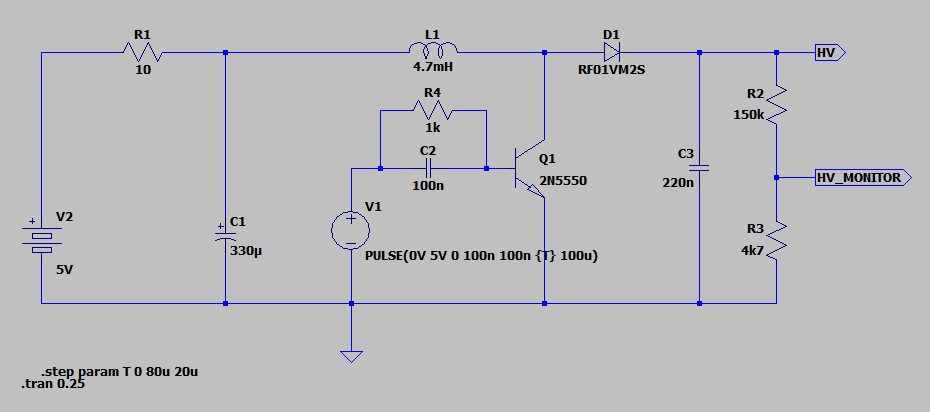
\includegraphics[width=\textwidth]{Spice/circuit.jpg}
            \caption[Simulated circuit of a boost converter.]{Simulated circuit of a boost converter using \textsc{LTspice}.}
            \label{fig:simCircuit}
        \end{figure}
        %
        \begin{figure}[h]
            \centering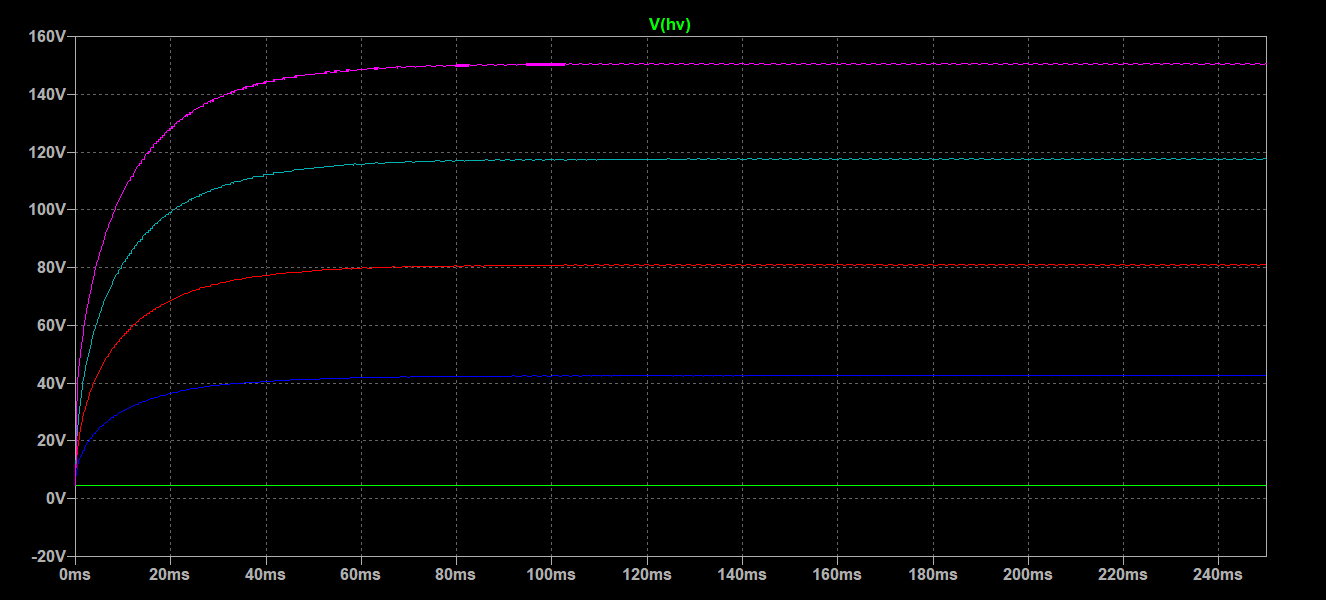
\includegraphics[width=\textwidth]{Spice/plot.jpg}
            \caption{Plot of the output voltage at \textit{HV}. The voltage is subsequently progressing towards a peak voltage of \( \hat{U}_{HV} \approx \SI[]{150}[]{V} \) with rising PWM duty cycle.}
            \label{fig:plotSimCircuit}
        \end{figure}
        %
    \subsection*{Charge/Discharge Time of a Capacitor}\label{sec:charge-discharge-time}
        %
        Charging:
        \begin{gather}
            U_{Br} = U_+ \left( 1 - e^{-\frac{t_{charge}}{R_6C_5}}\right) \nonumber \\
            \Leftrightarrow \nonumber \\
            t_{charge} = - \ln\left(1 - \frac{U_{Br}}{U_+}\right) \cdot R_6 C_5
            \label{eq:avalanche_charging_equation}
        \end{gather}
        Discharging:
        \begin{gather}
            U_{C_5} = U_{Br} \left(e^{-\frac{t_{discharge}}{R_7C_5}}\right) \nonumber \\
            \Leftrightarrow \nonumber \\
            t_{discharge} = -\ln\left( \frac{U_{C_5}}{U_{Br}} \right) \cdot R_7 C_5
            \label{eq:avalanche_discharging_equation}
        \end{gather}
        plugging in the values for \(U_{Br} = \SI{65}{V}, U_+ = \SI{75}{V}, U_{C_5} = \SI{5}{V}, C_5 = \SI{2.2}{pF}, R_6 = \SI{1}{M\ohm} \text{ and } R_7 = \SI{51}{\ohm}\)
        equates to the following charging/discharging times \(t_{charge}\) and \(t_{discharge}\):
        \begin{align}
            t_{charge} &= - \ln\left(1 - \frac{\SI{65}{V}}{\SI{75}{V}}\right) \cdot \SI{10^6}{\ohm} \cdot \SI{2.2 \cdot 10^{-12}}{F} \nonumber \\
            &\approx \SI{4.43 \cdot 10^{-6}}{s} \label{eq:avalanche_charging_time}\\
            \nonumber \\
            t_{discharge} &= -\ln\left( \frac{\SI{5}{V}}{\SI{65}{V}} \right) \cdot \SI{51}{\ohm} \cdot \SI{2.2 \cdot 10^{-12}}{F} \nonumber \\
            &\approx \SI{2.88 \cdot 10^{-10}}{s} \label{eq:avalanche_discharging_time}
        \end{align}
        With these numbers, the minimum time per charge/discharge cycle would be the sum of both times. Thus, the maximum number
        of repetitions per second \(f_{Rep}\) is
        \begin{equation}
            f_{Rep} = \left(t_{charge} + t_{discharge}\right)^{-1} \approx \SI{225.7}{kHz}
        \end{equation}
        %
    \subsection*{Cable Characteristics of RG-58/U Coaxial Cable}% A4
        %
        Nominal characteristic impedance: \(\SI{53}{\ohm}\)\par
        Nominal velocity of propagation: \(69.5\%\)\par
        Nominal delay (translates to the inverse of the absolute speed of propagation): \(\SI{4.85588}{\nicefrac{ns}{m}}\)\par
        The values above are taken from the technical data sheet \cite{Belden.RG-58/U.CoaxCable.Datasheet}.
        %
    \subsection*{Determining the Suitability of the Oscilloscope}% A5
        %
        The oscilloscope at hand is labeled with a bandwidth of \( B = \SI{200}{MHz} \). Following \cref{eq:bandwidth_and_riseTime}
        edges faster than
        \begin{equation}
            t_{rise_{min}} \approx \frac{0.35}{\SI{200}{MHz}} \approx \SI{1.75}{ns}
        \end{equation}
        %
    \subsection*{Sampling Rate}% A6
    %
    %